%
%  This is an example LaTeX file. The percent sign is used to mark the
% start of a comment.
%
%  - Michael Weeks,  January, 2003
%
\documentclass[10pt]{article}
\usepackage[a4paper, total={6in, 8in}]{geometry}
\usepackage{rotating,graphicx}
\usepackage[hidelinks]{hyperref}
\usepackage{lscape}
\usepackage{listings}
\usepackage{float}
\hypersetup{
  colorlinks   = true,    % Colours links instead of ugly boxes
  urlcolor     = blue,    % Colour for external hyperlinks
  linkcolor    = blue,    % Colour of internal links
  citecolor    = red      % Colour of citations
}

%\journal{CSc 4110 Final Report}

%\title[journalExample]{Format for Project Reports}
\title{Engineering Update on the project: \textit{\textbf{"EEG Measures for Schizophrenia"}}}
%\author{%
%Dr. K.P. Ayodele, Emmanuel OLATEJU \\
%    \begin{affiliation}
%      Excelsiors \\ 09/02/2023, \\
 %     email: \mbox{kayodele@gmail.com, eoolateju@student.oauife.edu.ng}
%      \end{affiliation}
%}


\begin{document}



\maketitle

\section{Summary}
MMN computation has been altered to be referenced to the standard tone, include min-max scaling and use of a five point moving average for plotting.
This improved visual interpretation of the waveforms. The figures are shown in section \ref{sec:figures}.\\
\\
Fuzzy entropy computation now add extras space dimensions whose signal is a gaussian noise of a unit standard deviation.
So there is no need for combination of electrode from corticla regions to compute fuzzy entropy anymore.\\
\\
A fuzzy entropy algorithm for a univariate time-series has been implemented and tested. The algorithm 
is to be improved by being extended for a multivariate time -series(2D data). This algorithm is shown in \ref{sec:appendix}.\\
\\
Further data has been acquired from 20 more subjects. This data is not included yet. The new data recordings will be included 
in future processing and reports.\\
\\
An handheld annotator is being developed for easy feedback to DAQ system from patient and  
clinician.

\section{Next Steps}
Over the period of four weeks, I will be doing the following
\begin{itemize}
  \item Continued development of hand held annotator device.
  \item Computing MMN amplitudes from the MMN waveforms.
  \item Improving self-developed fuzzy entropy library to work with multivariate
  time-series(2D data).
  \item Recomputing fuzzy entropy features.
  \item Comparing fuzzy entropy features from developed library to sourced library.
  \item Computing auditory steady state response and features.
\end{itemize}
            

\section{Figures}\label{sec:figures}
\begin{figure}[H]
  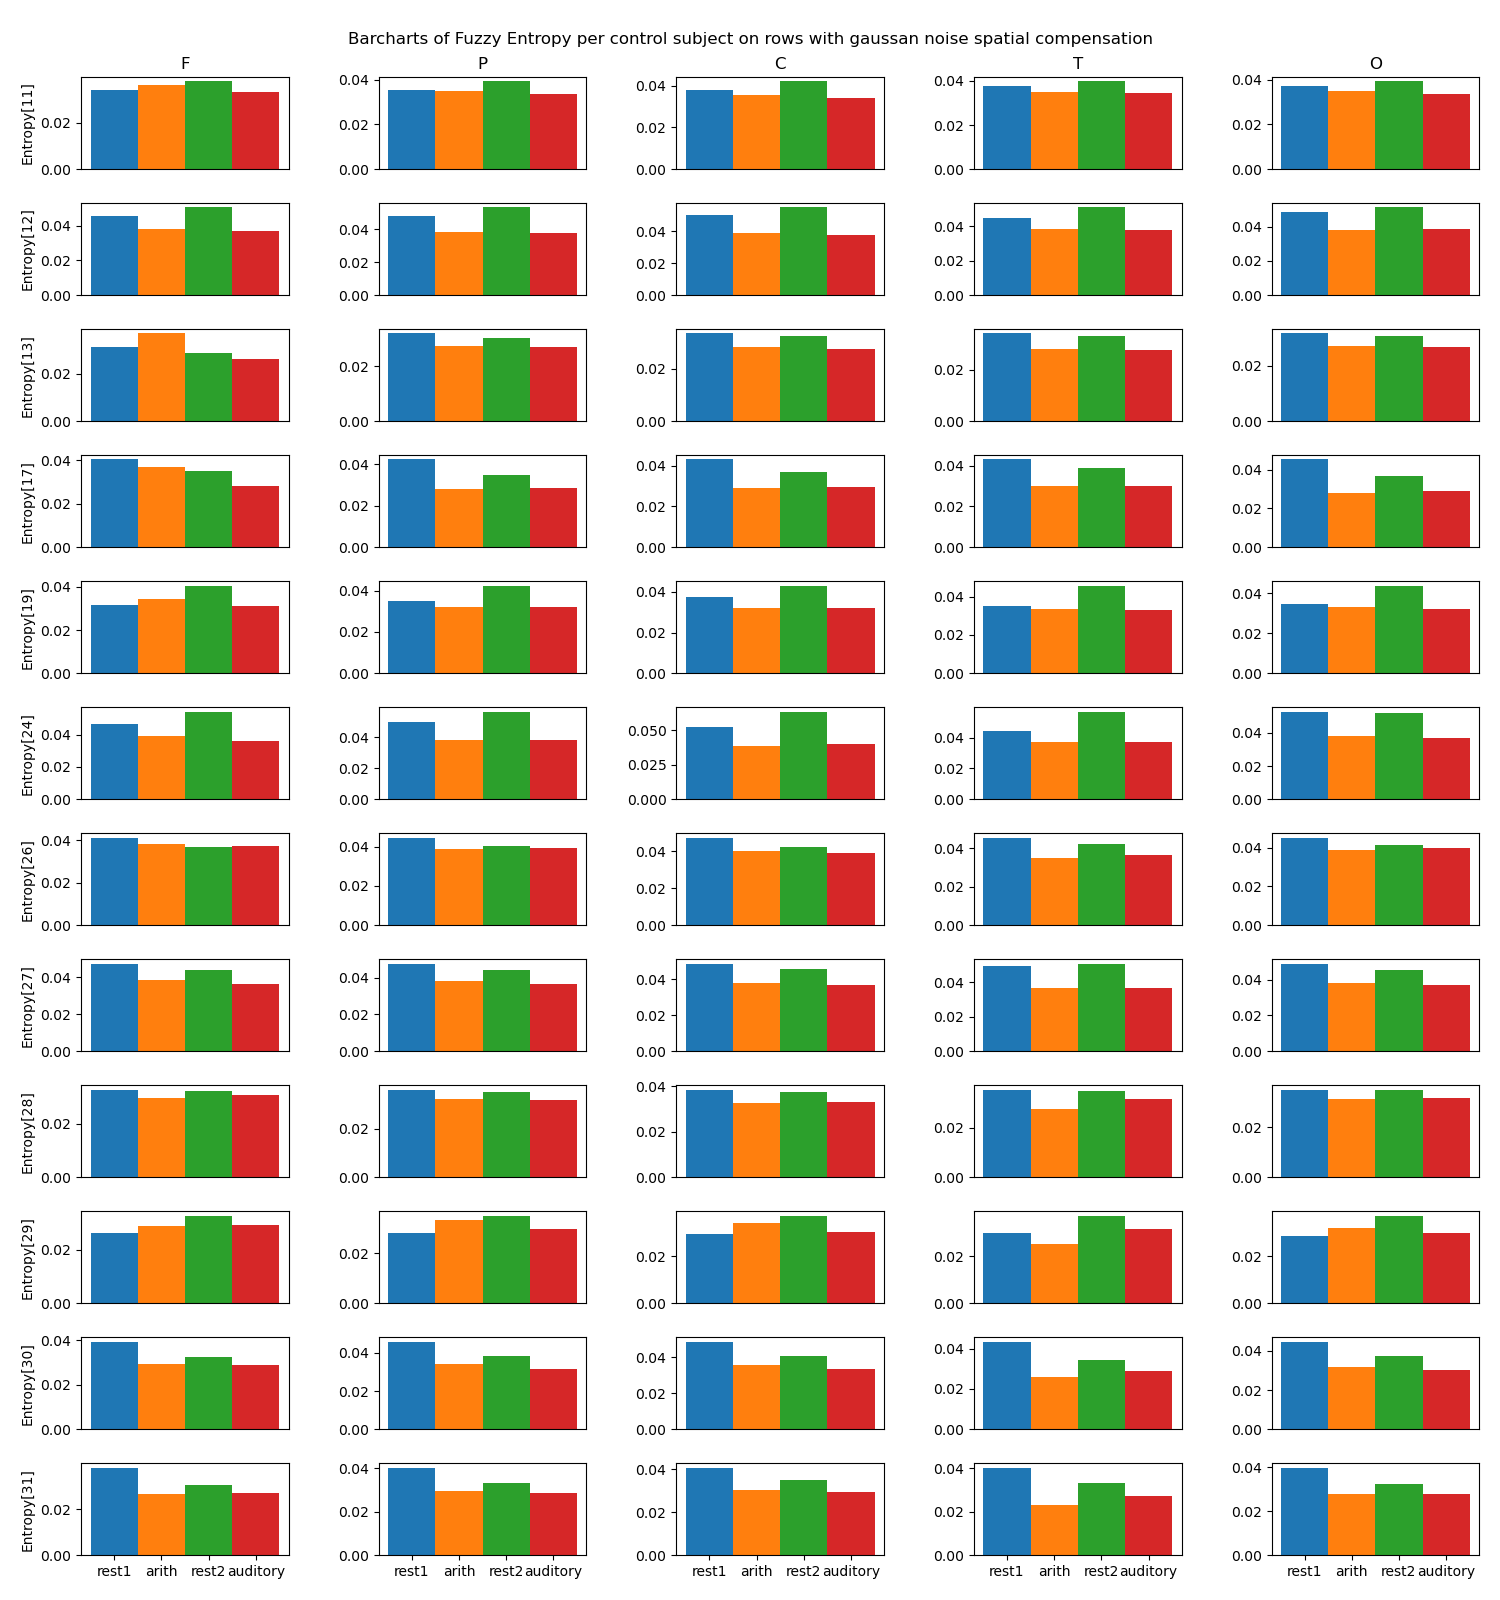
\includegraphics[width=16cm]{../../../data_analysis_results/FuzzEnt/Control/all-fuzzyEntr.png}
  \caption{Fuzzy Entropy from controls}
  \label{fig:controlFuzzEnt}
\end{figure}

\begin{figure}[H]
  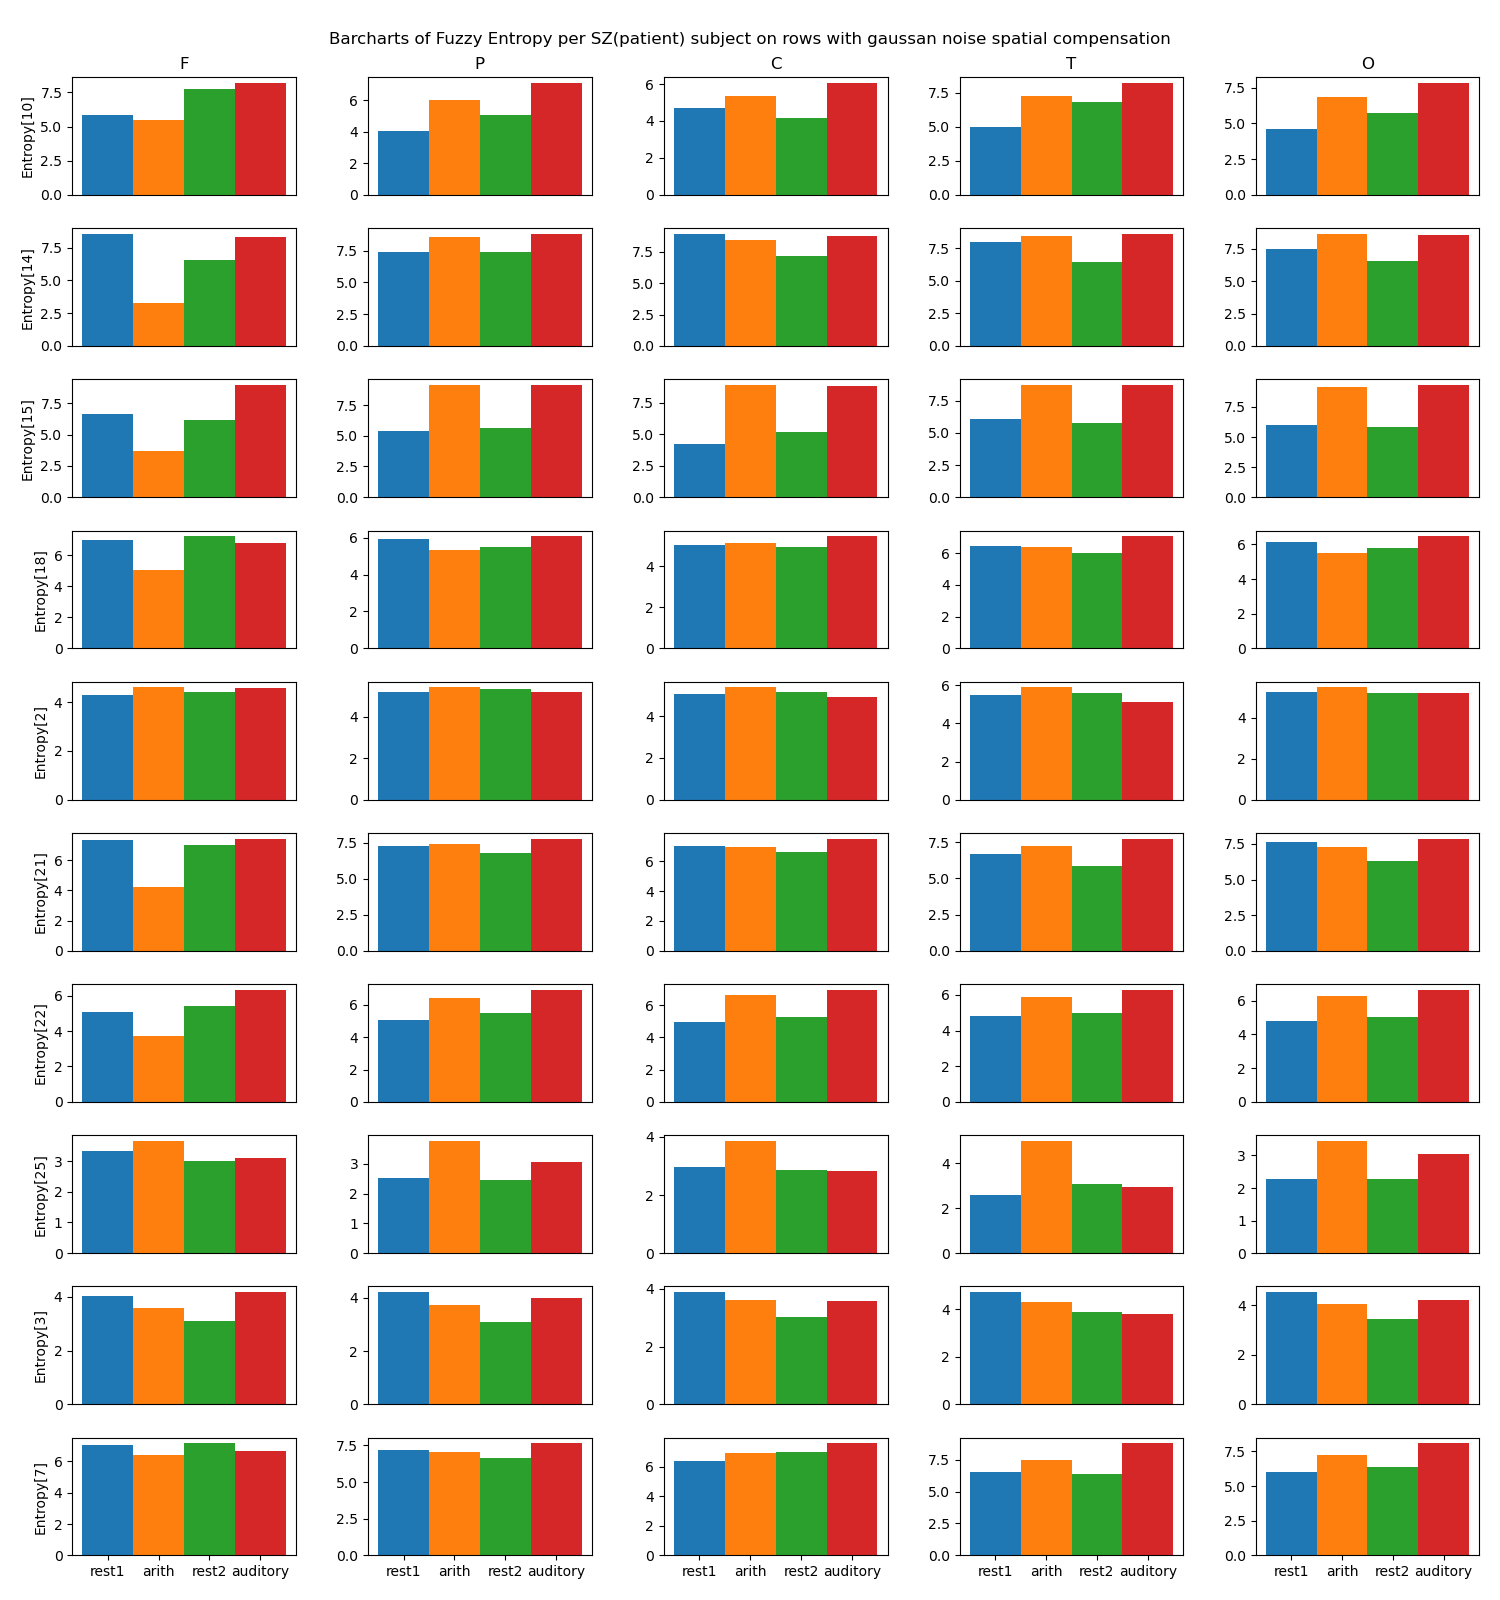
\includegraphics[width=16cm]{../../../data_analysis_results/FuzzEnt/Patient/all-fuzzyEntr.png}
  \caption{Fuzzy Entropy from patients}
  \label{fig:patientFuzzEnt}
\end{figure}

\begin{figure}[H]
  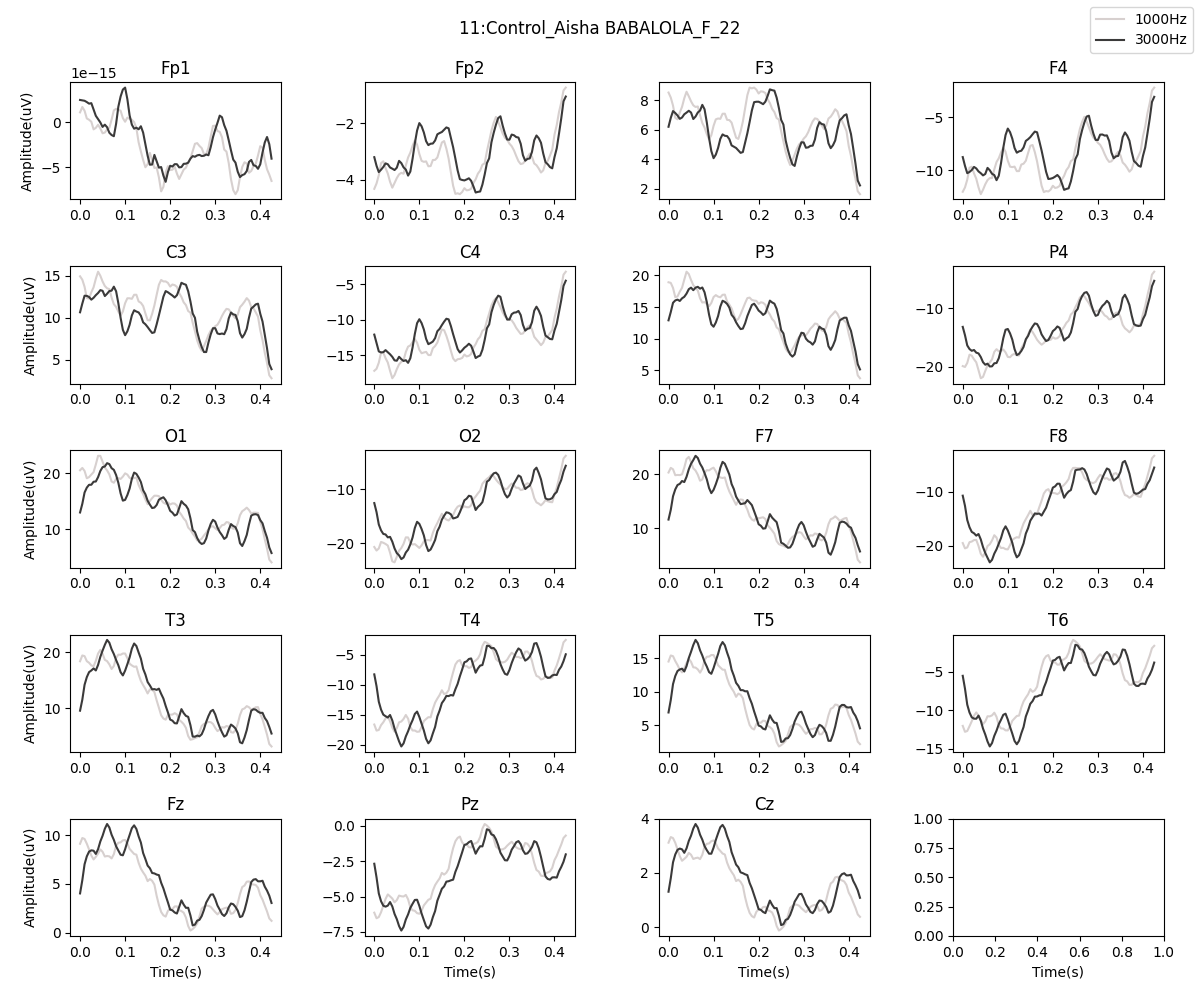
\includegraphics[width=16cm]{../../../data_analysis_results/MMN/time_series/Control/11.png}
  \caption{A control subject MMN plots}
\end{figure}
\begin{figure}[H]
  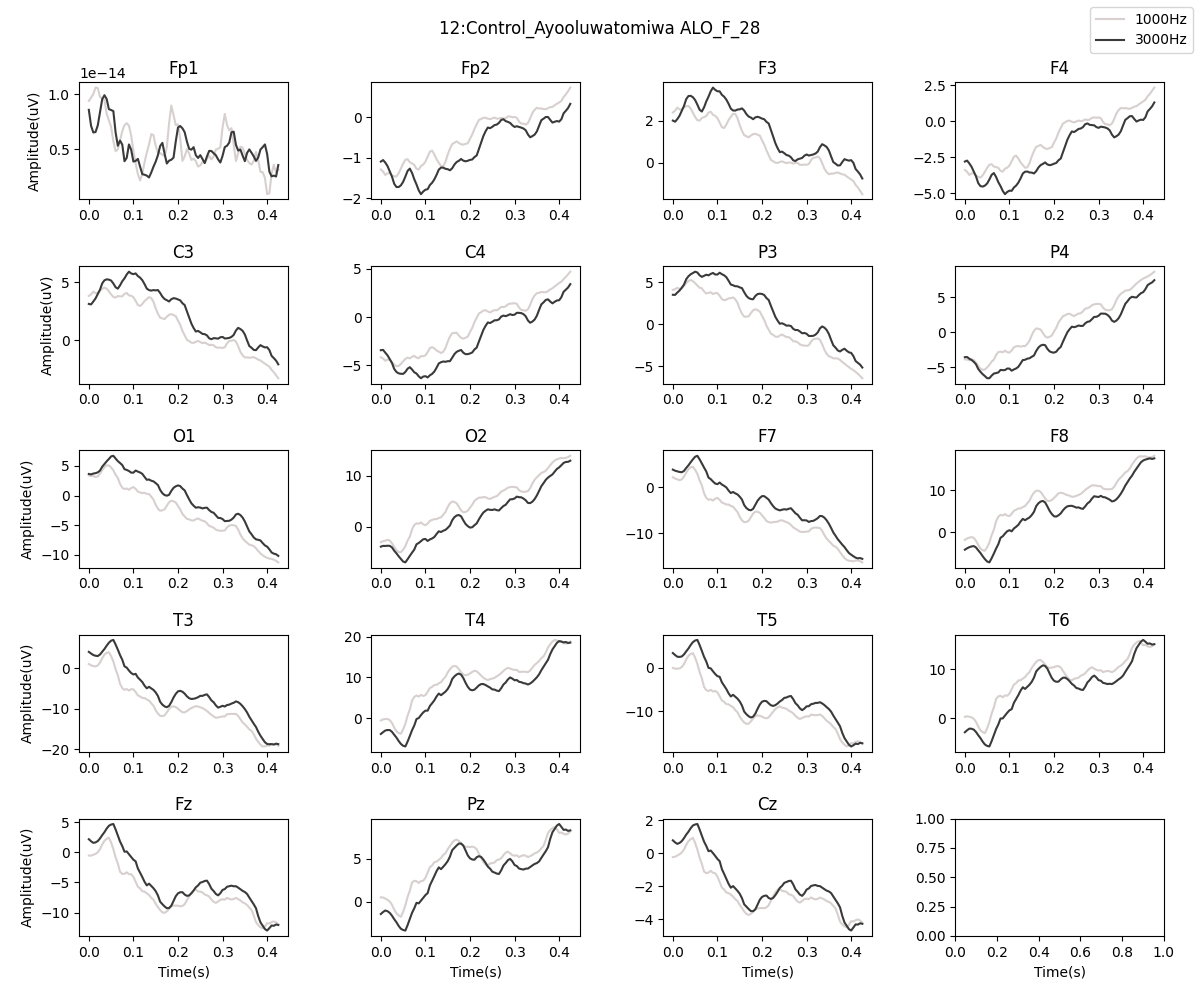
\includegraphics[width=16cm]{../../../data_analysis_results/MMN/time_series/Control/12.png}
  \caption{A control subject MMN plots}
\end{figure}
\begin{figure}[H]
  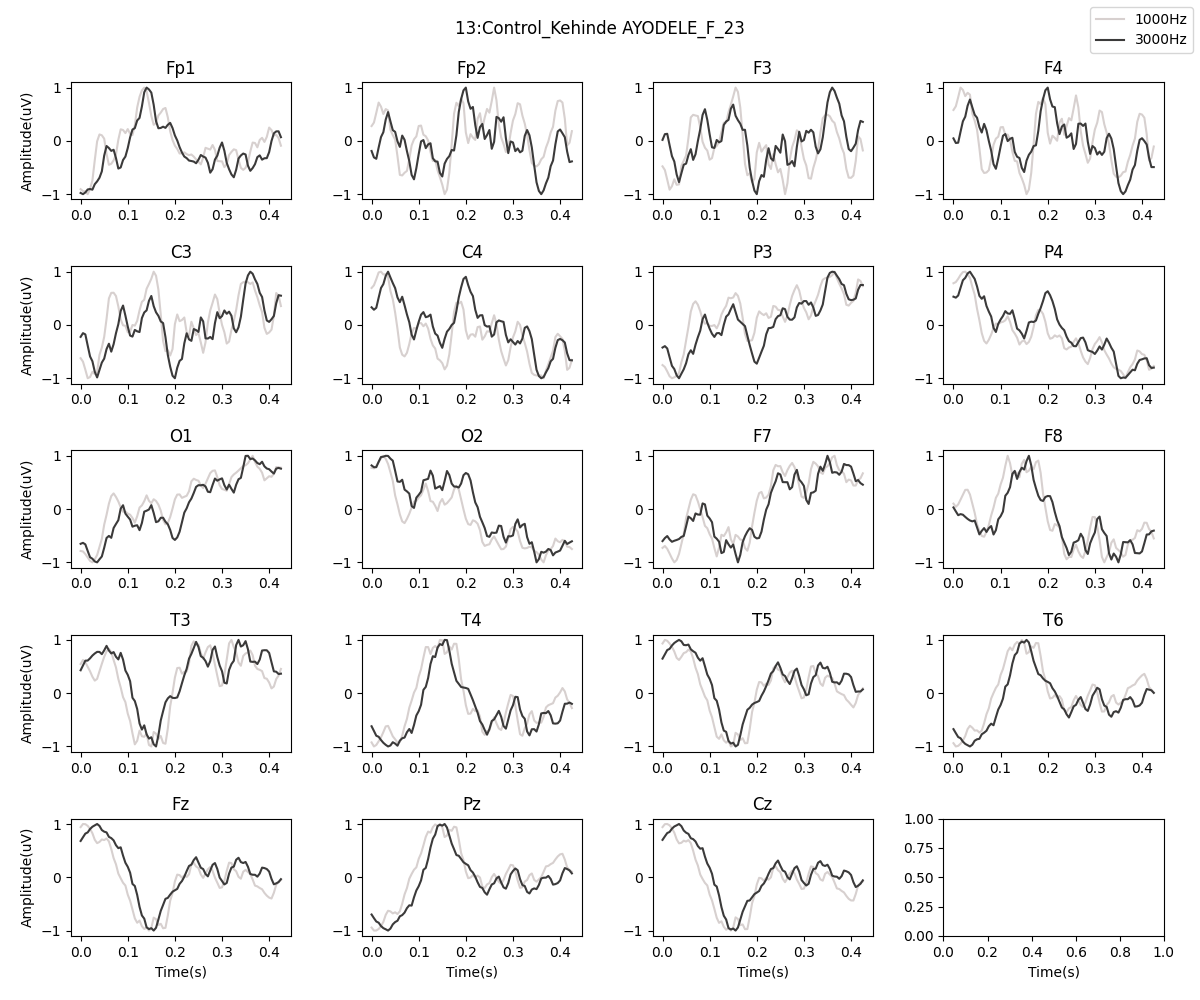
\includegraphics[width=16cm]{../../../data_analysis_results/MMN/time_series/Control/13.png}
  \caption{A control subject MMN plots}
\end{figure}
\begin{figure}[H]
  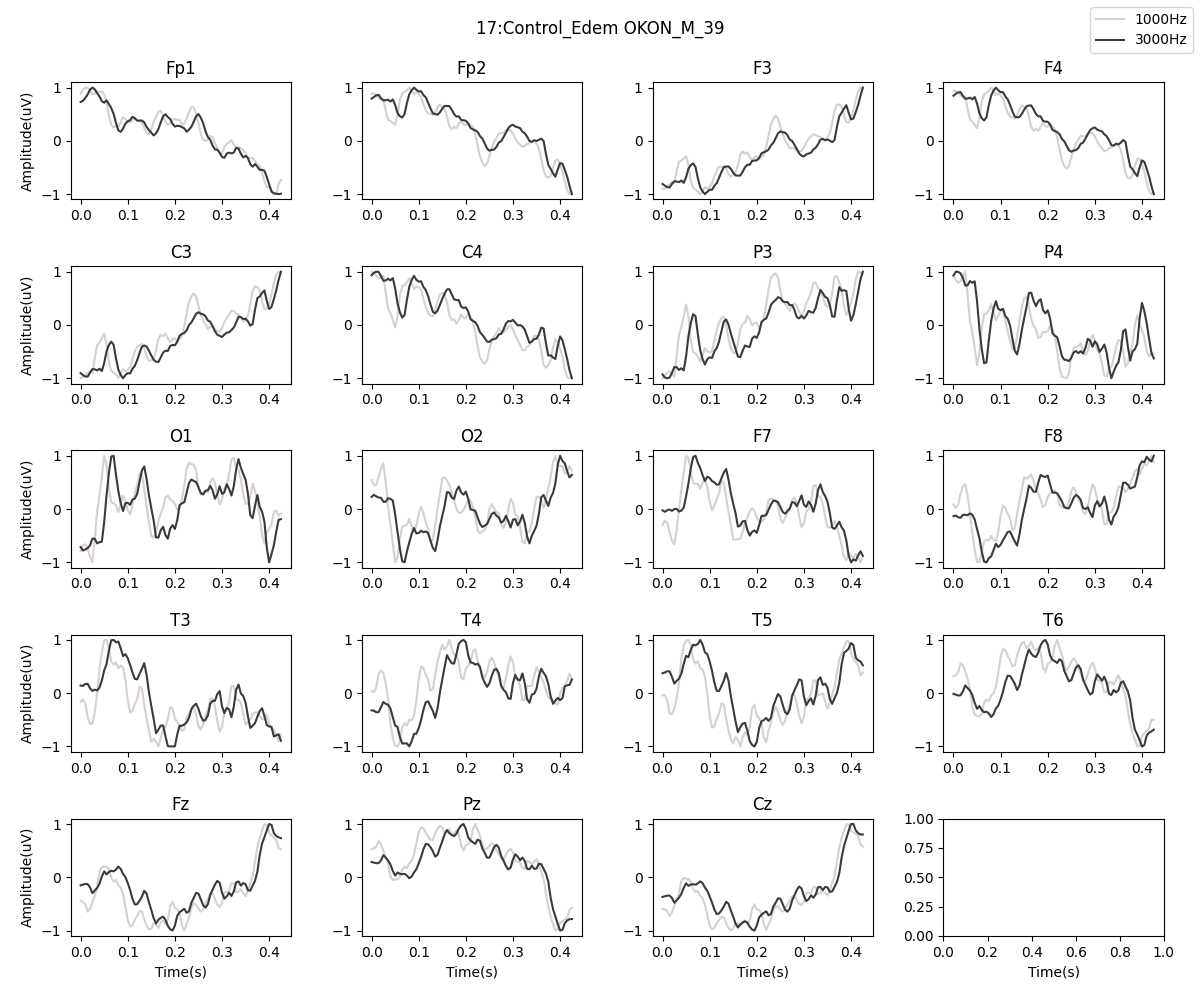
\includegraphics[width=16cm]{../../../data_analysis_results/MMN/time_series/Control/17.png}
  \caption{A control subject MMN plots}
\end{figure}
\begin{figure}[H]
  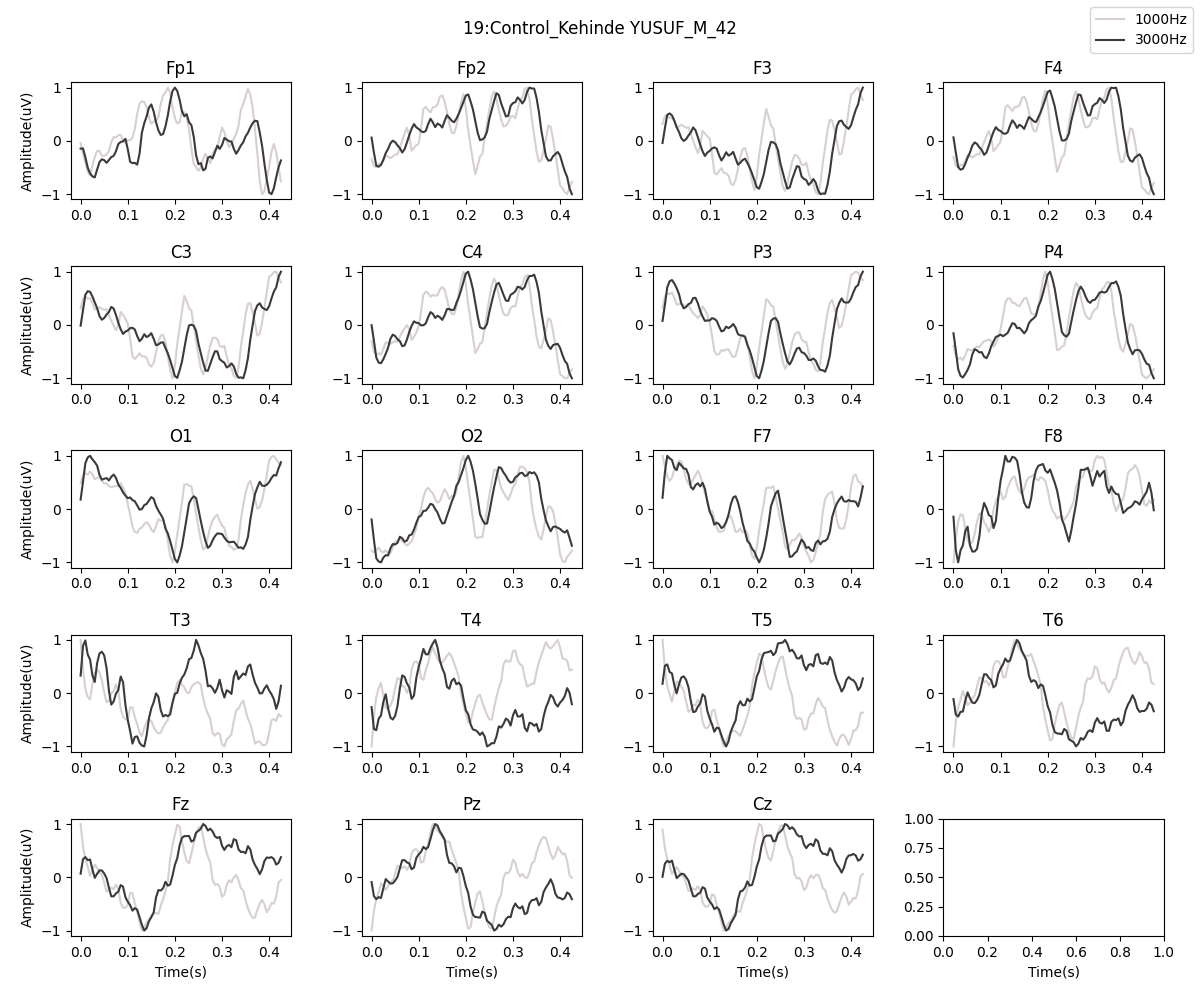
\includegraphics[width=16cm]{../../../data_analysis_results/MMN/time_series/Control/19.png}
  \caption{A control subject MMN plots}
\end{figure}
\begin{figure}[H]
  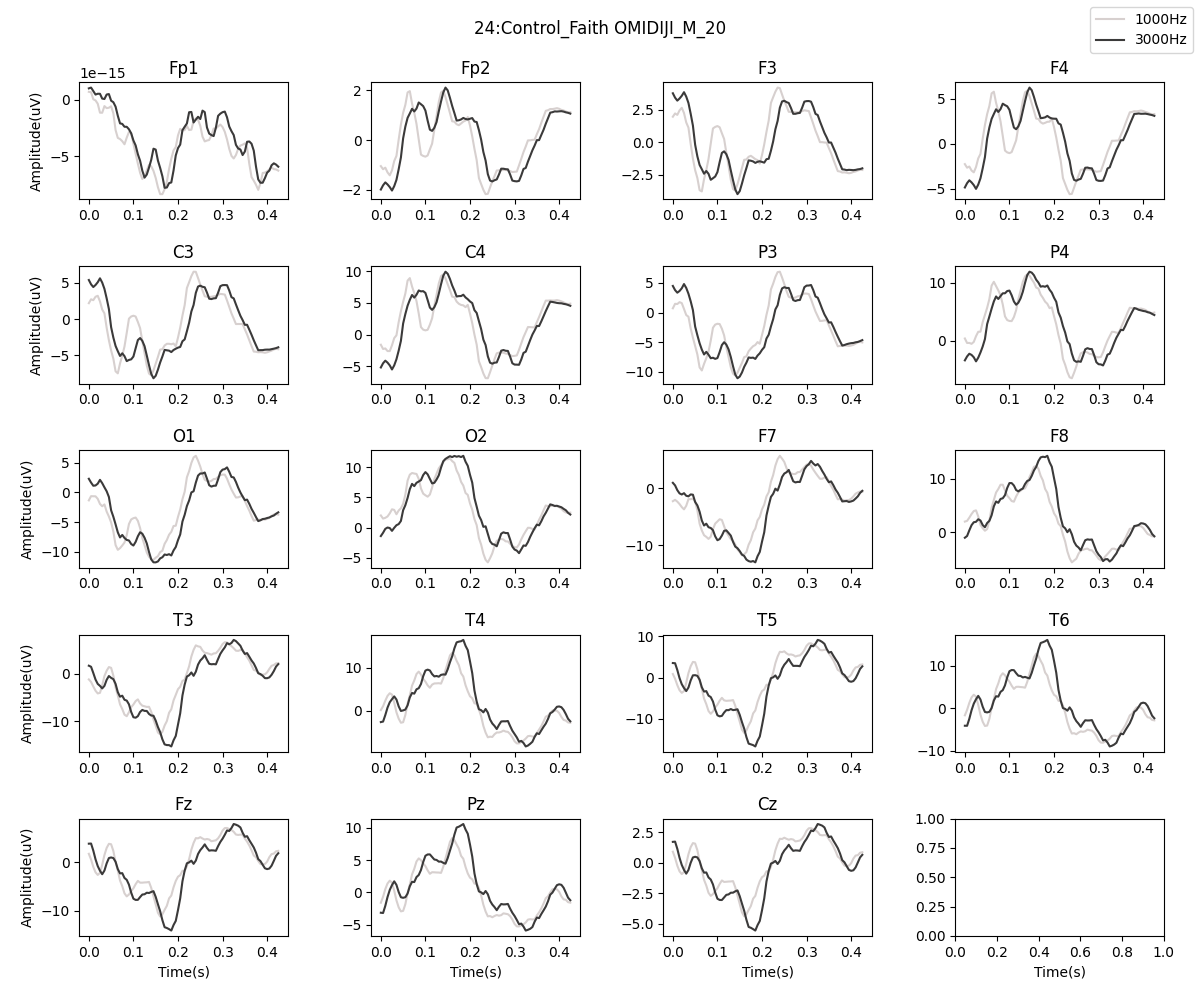
\includegraphics[width=16cm]{../../../data_analysis_results/MMN/time_series/Control/24.png}
  \caption{A control subject MMN plots}
\end{figure}
\begin{figure}[H]
  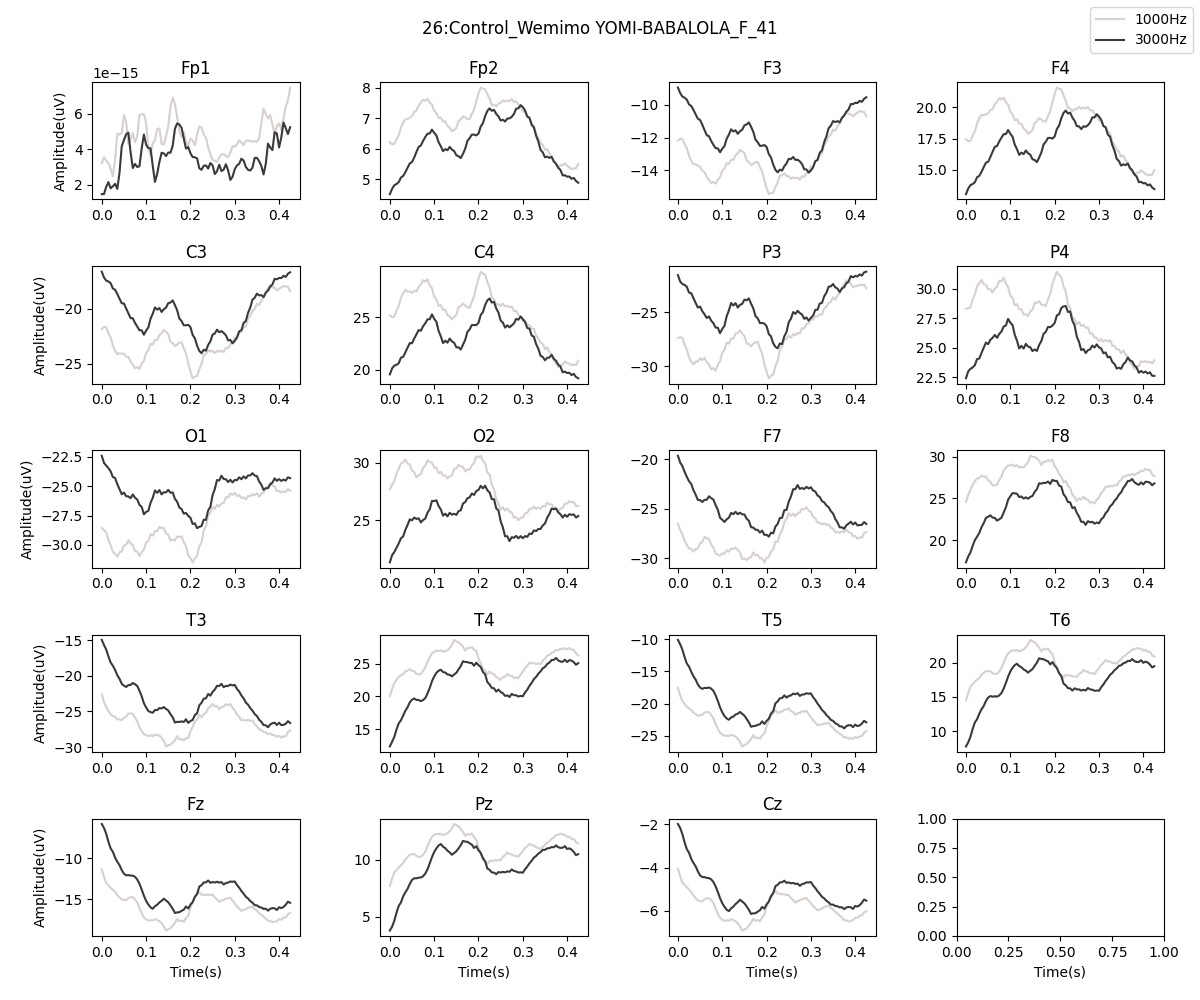
\includegraphics[width=16cm]{../../../data_analysis_results/MMN/time_series/Control/26.png}
  \caption{A control subject MMN plots}
\end{figure}
\begin{figure}[H]
  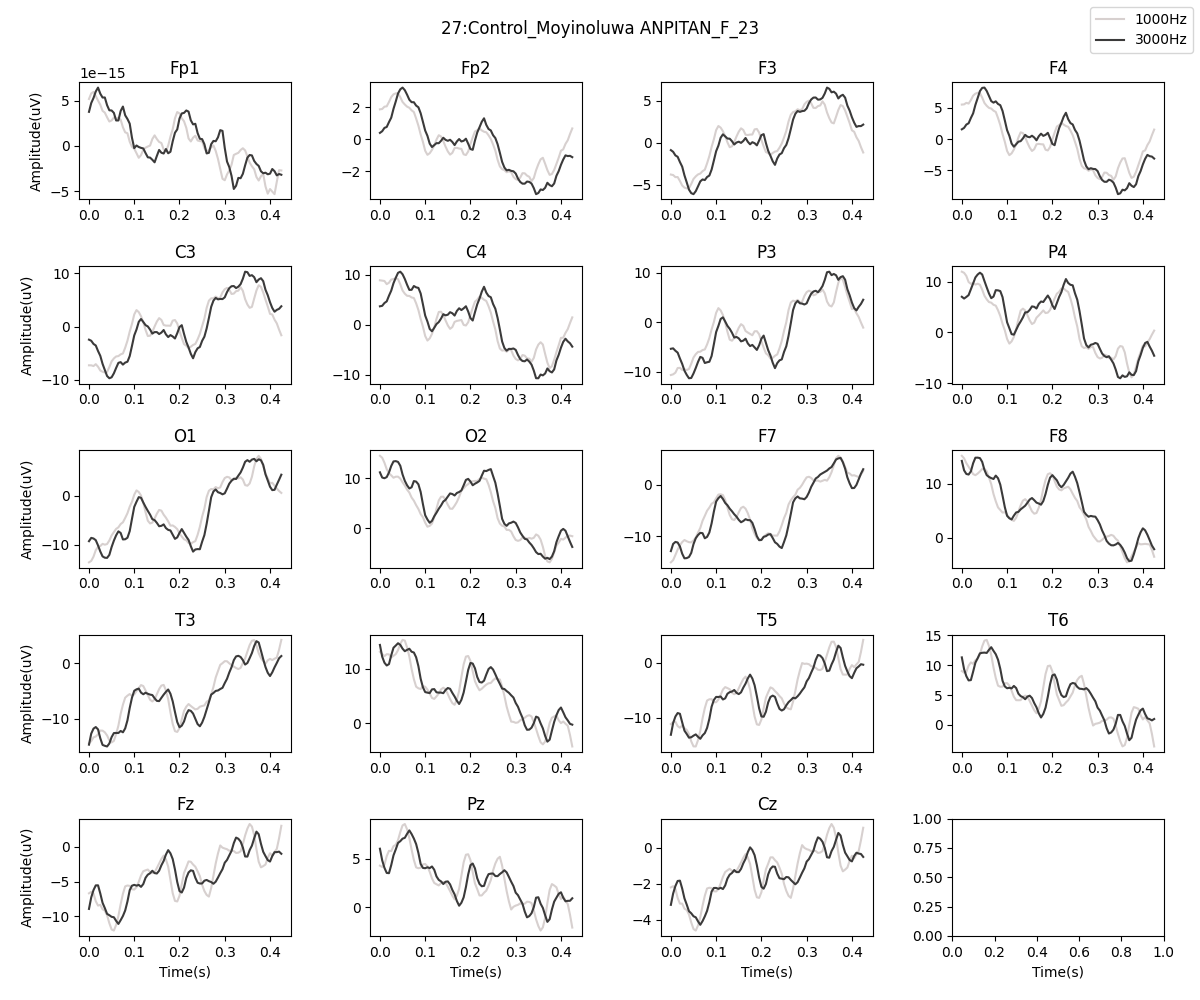
\includegraphics[width=16cm]{../../../data_analysis_results/MMN/time_series/Control/27.png}
  \caption{A control subject MMN plots}
\end{figure}
\begin{figure}[H]
  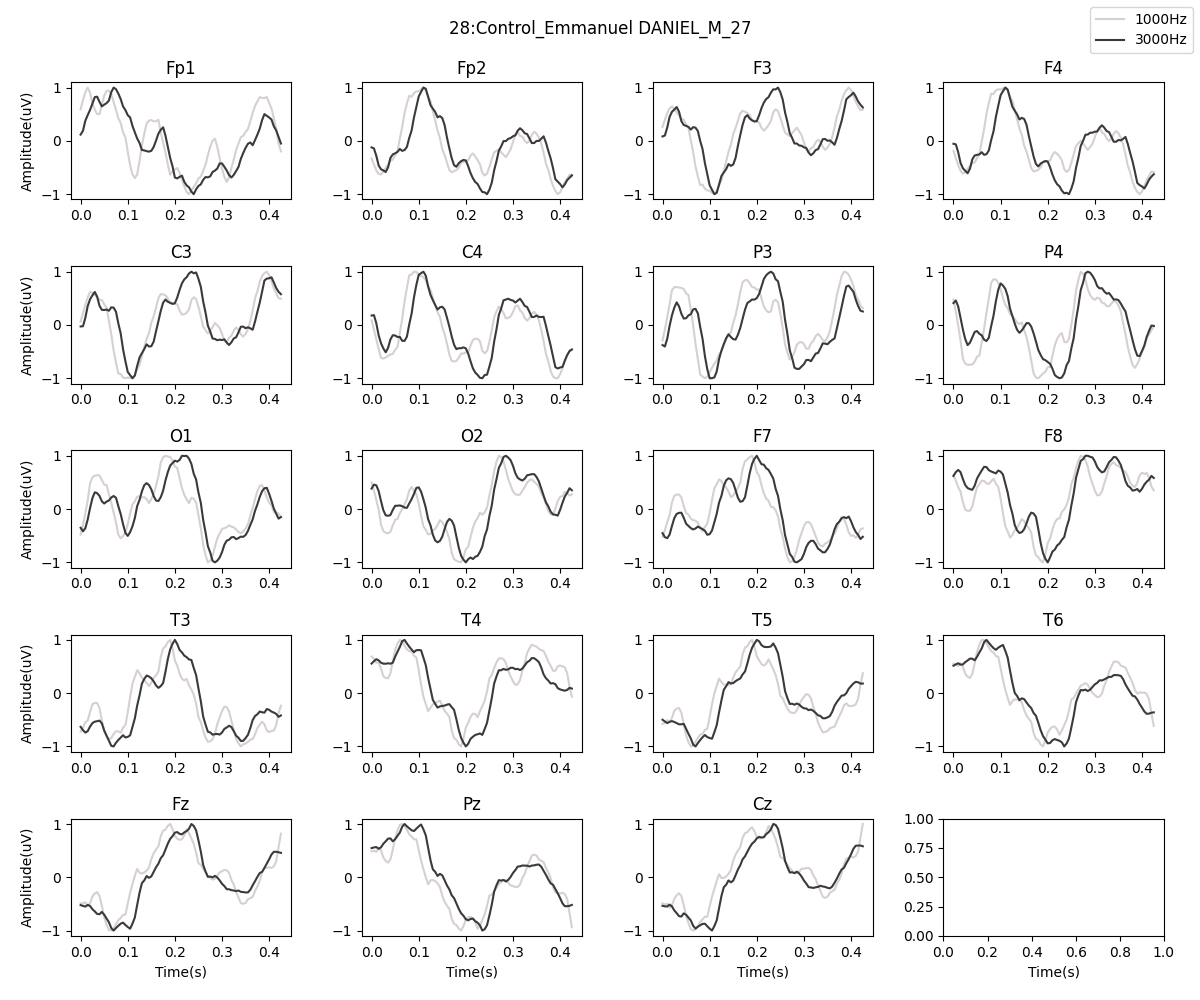
\includegraphics[width=16cm]{../../../data_analysis_results/MMN/time_series/Control/28.png}
  \caption{A control subject MMN plots}
\end{figure}
\begin{figure}[H]
  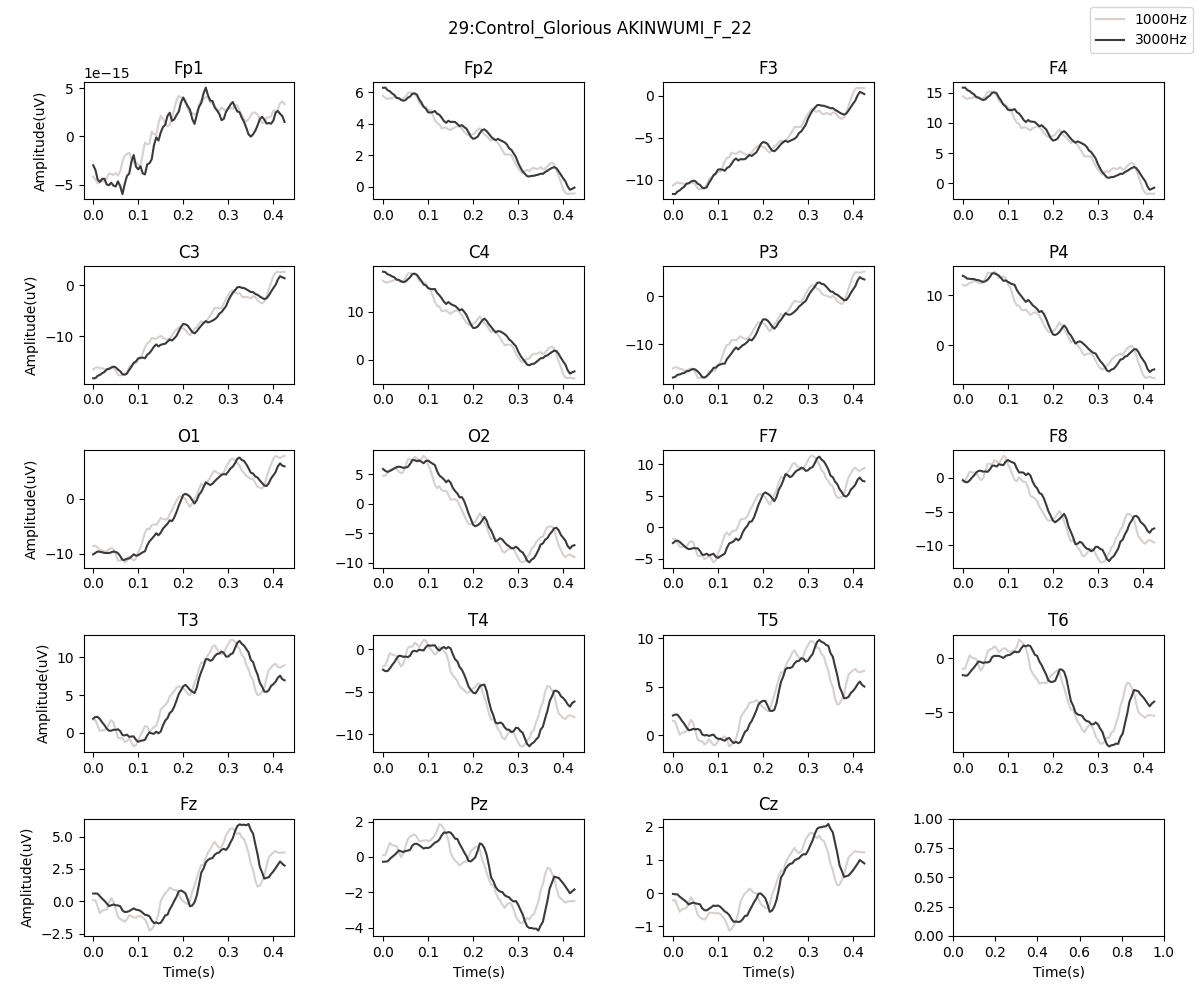
\includegraphics[width=16cm]{../../../data_analysis_results/MMN/time_series/Control/29.png}
  \caption{A control subject MMN plots}
\end{figure}
\begin{figure}[H]
  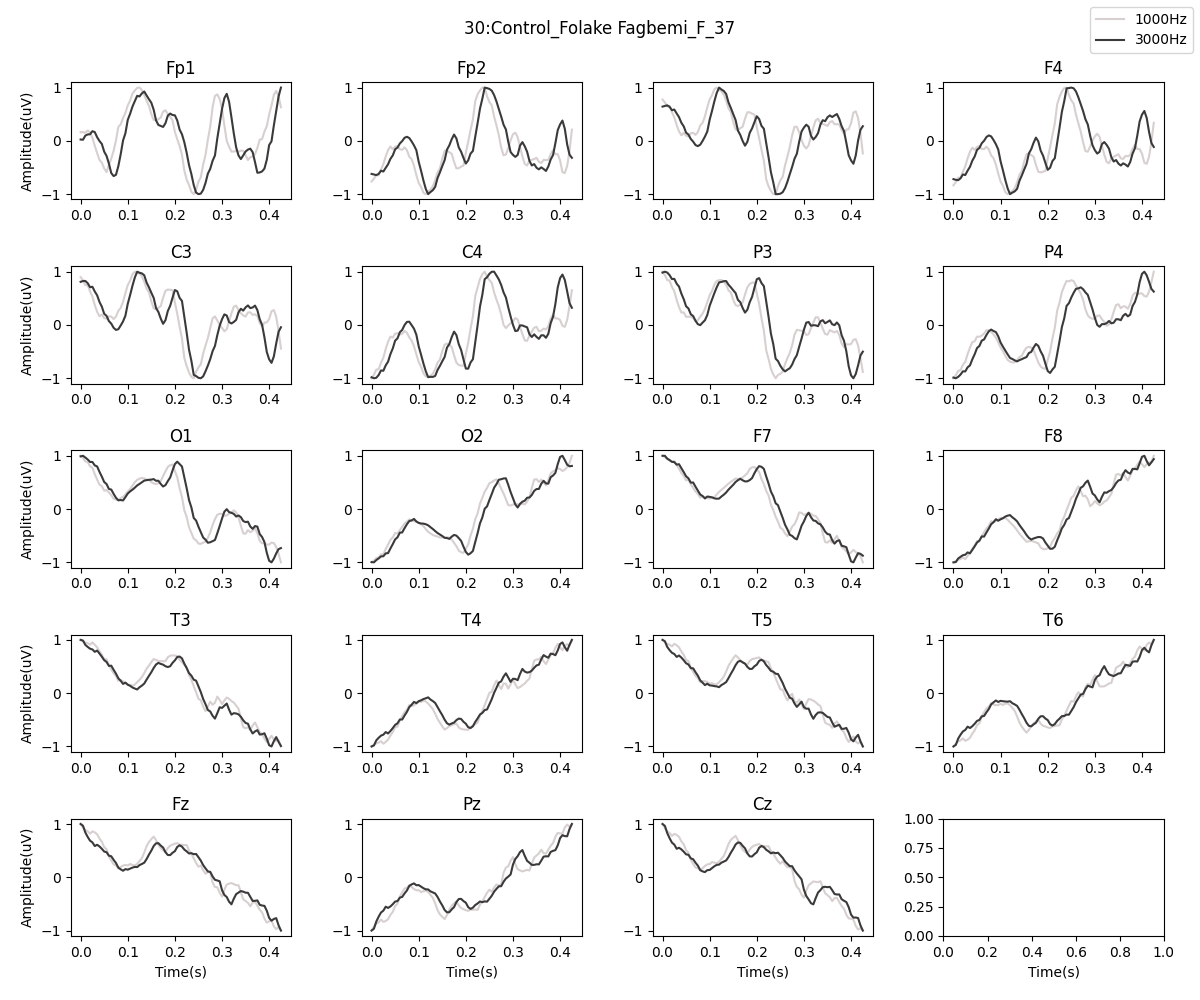
\includegraphics[width=16cm]{../../../data_analysis_results/MMN/time_series/Control/30.png}
  \caption{A control subject MMN plots}
\end{figure}
\begin{figure}[H]
  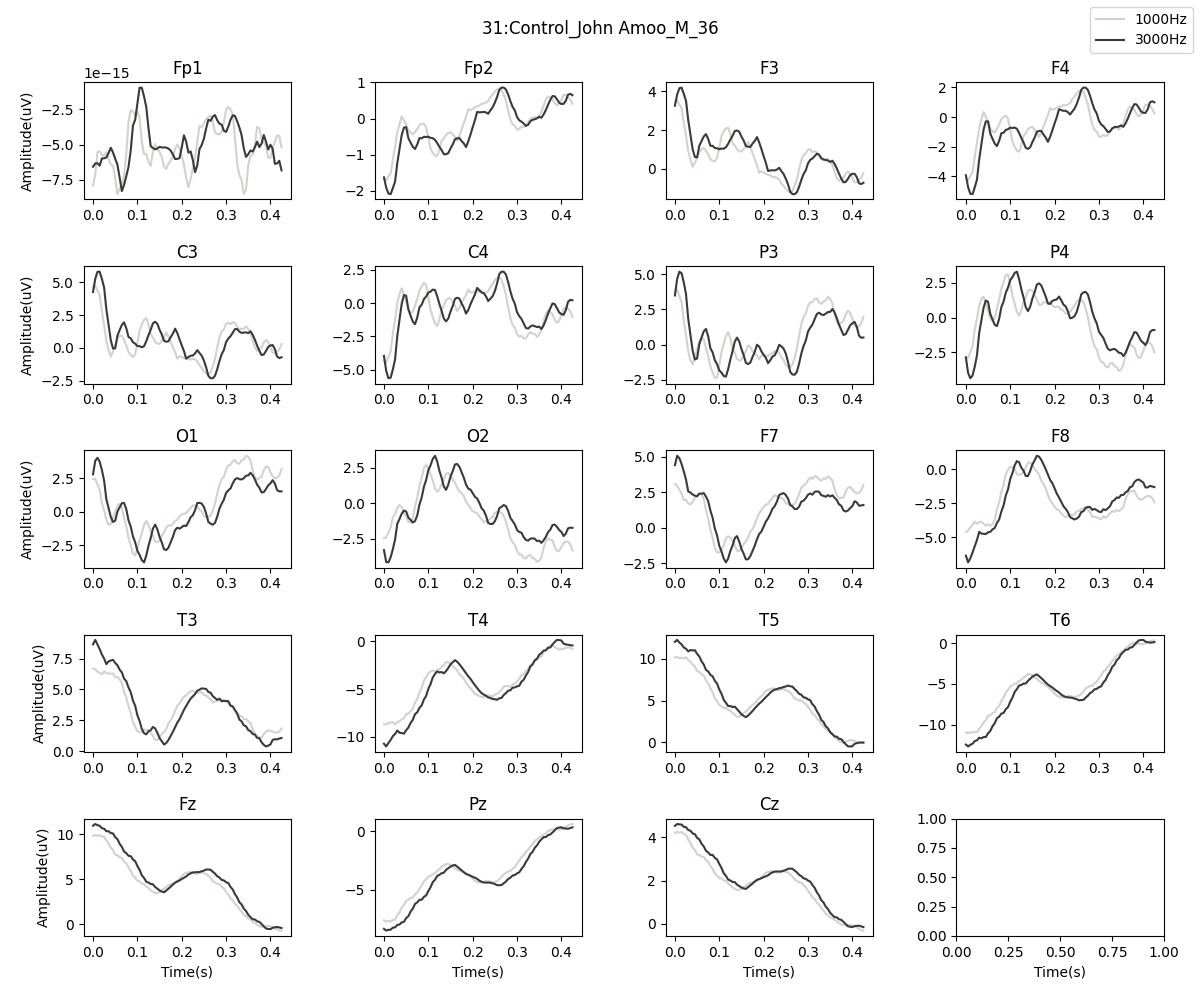
\includegraphics[width=16cm]{../../../data_analysis_results/MMN/time_series/Control/31.png}
  \caption{A control subject MMN plots}
\end{figure}


\begin{figure}[H]
  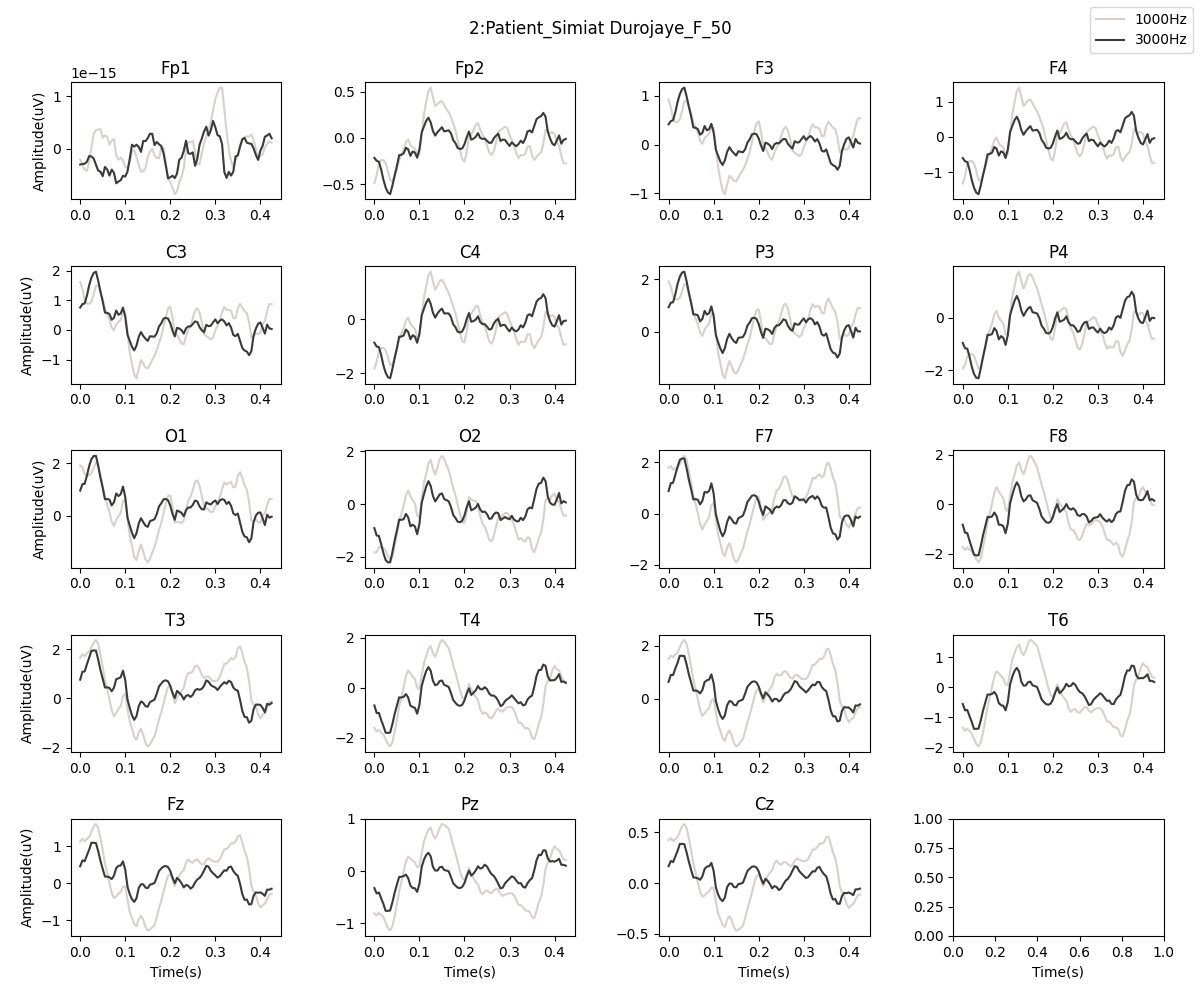
\includegraphics[width=16cm]{../../../data_analysis_results/MMN/time_series/Patient/2.png}
  \caption{A SZ subject MMN plots}
\end{figure}
\begin{figure}[H]
  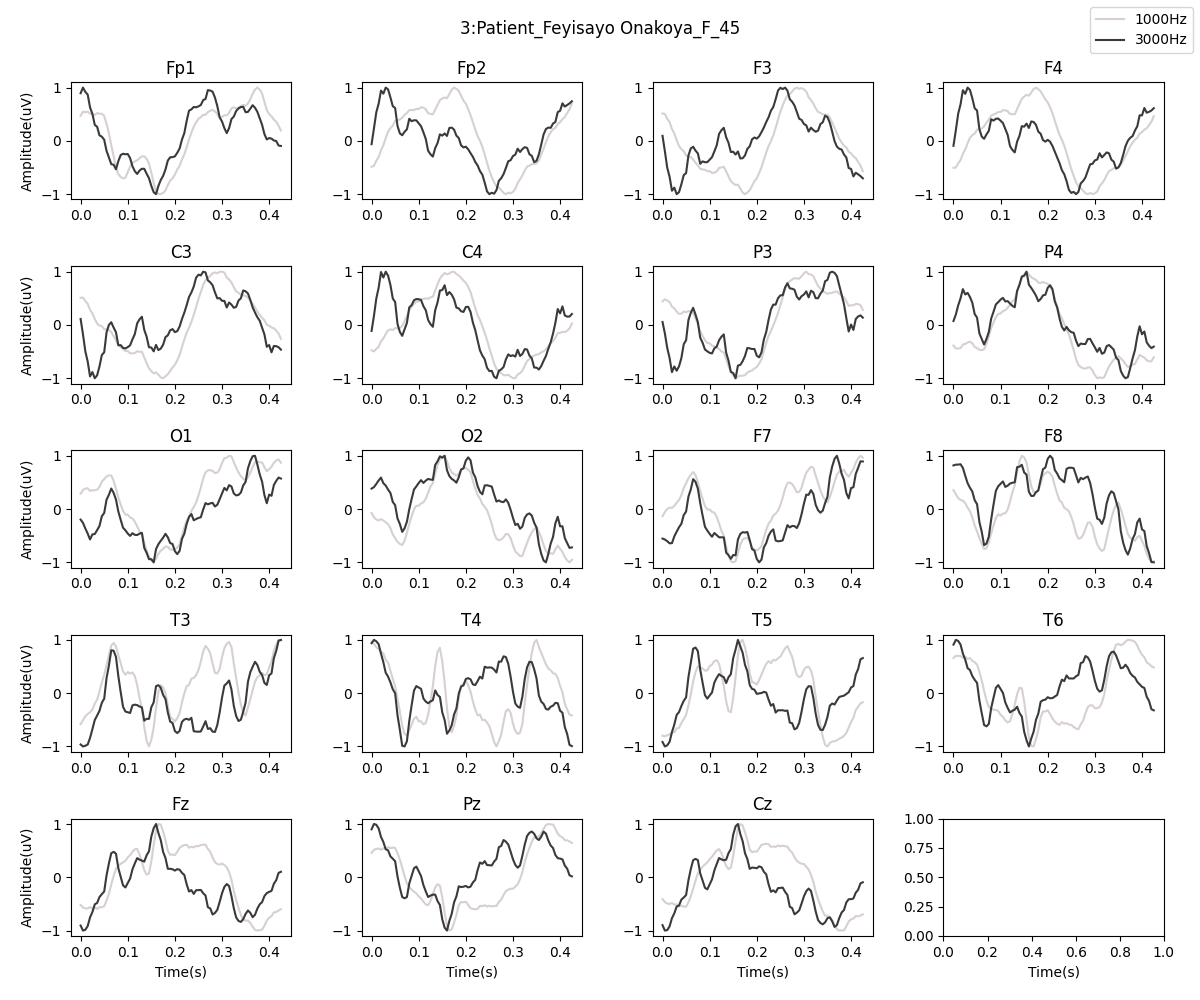
\includegraphics[width=16cm]{../../../data_analysis_results/MMN/time_series/Patient/3.png}
  \caption{A SZ subject MMN plots}
\end{figure}
\begin{figure}[H]
  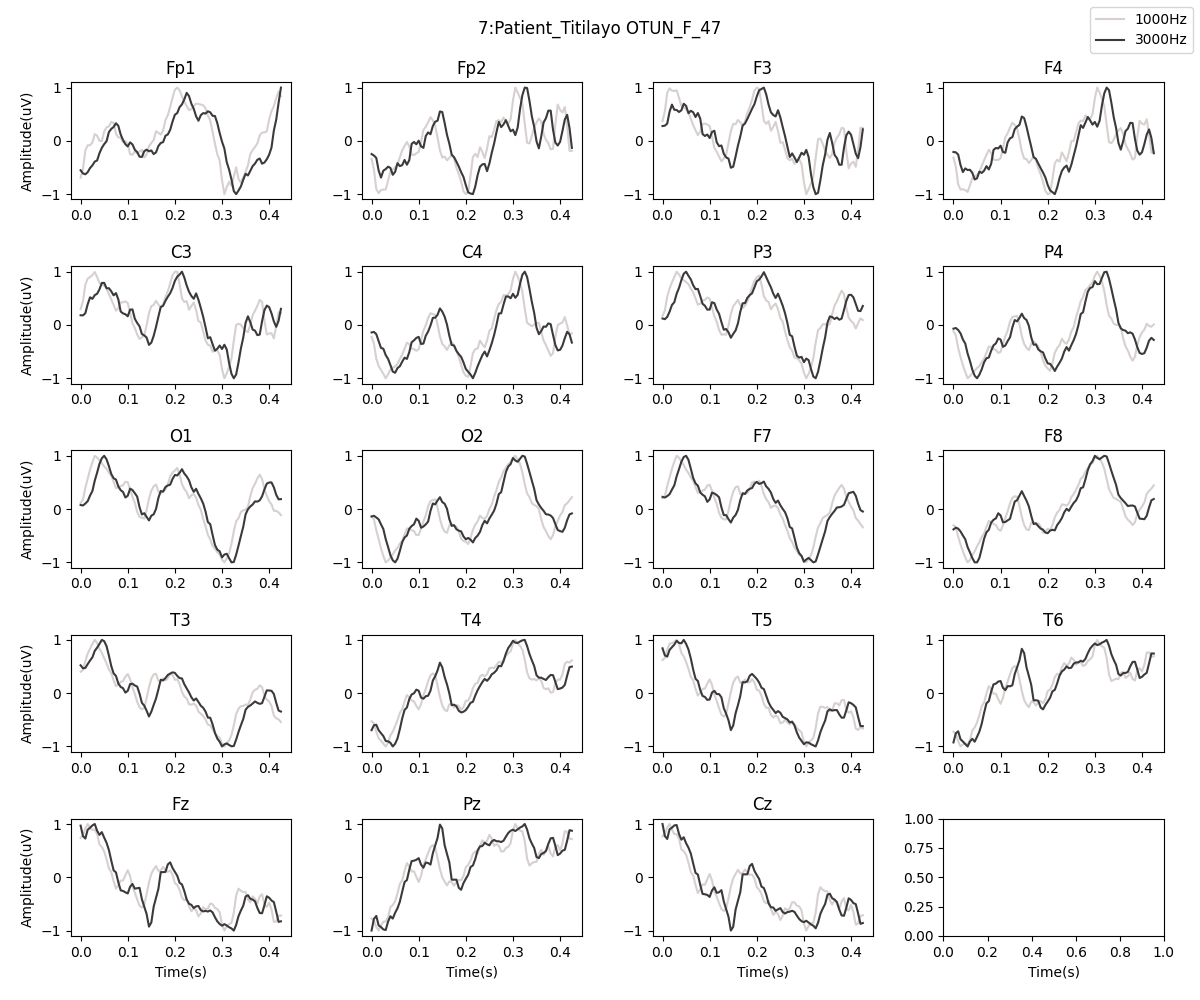
\includegraphics[width=16cm]{../../../data_analysis_results/MMN/time_series/Patient/7.png}
  \caption{A SZ subject MMN plots}
\end{figure}
\begin{figure}[H]
  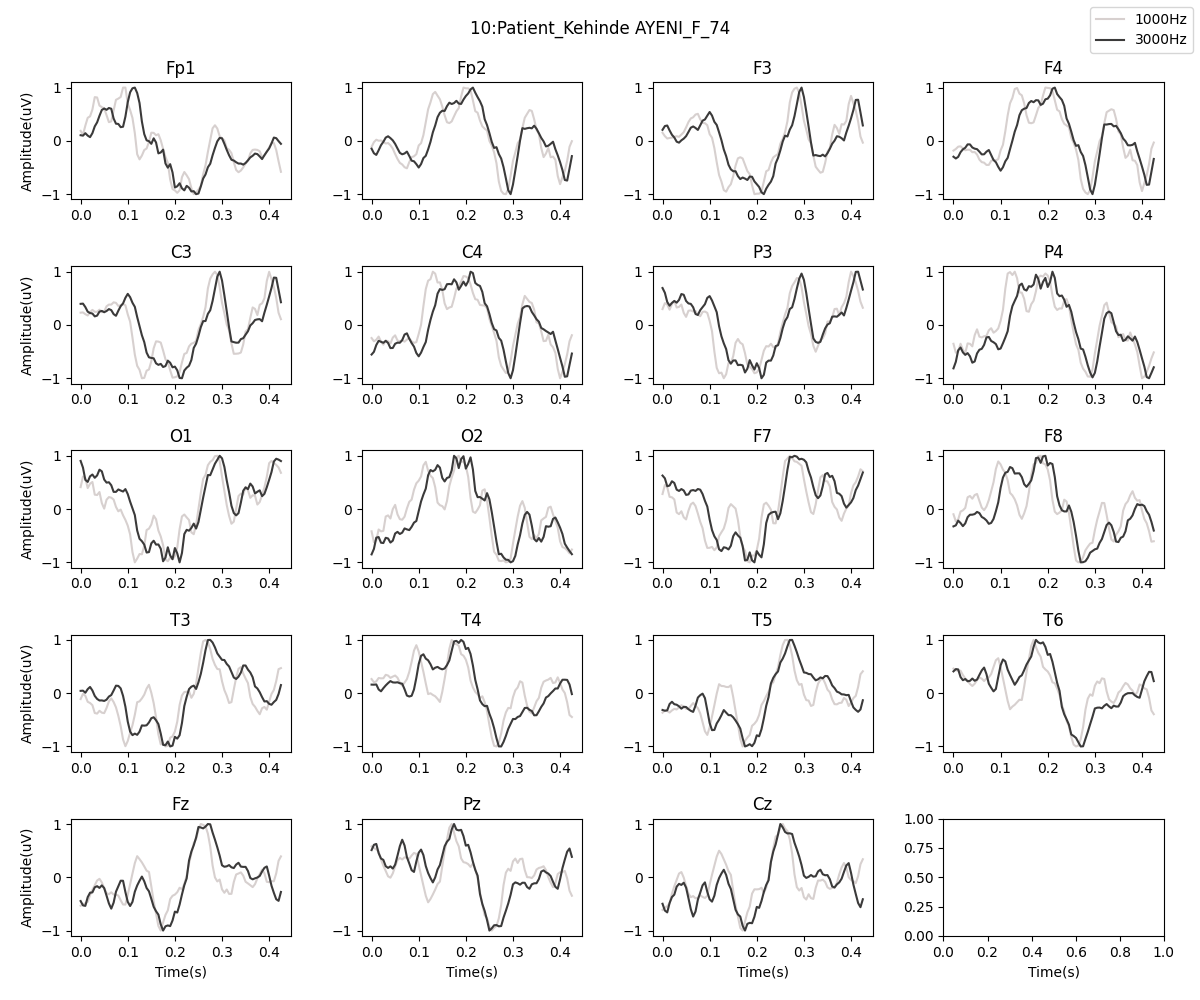
\includegraphics[width=16cm]{../../../data_analysis_results/MMN/time_series/Patient/10.png}
  \caption{A SZ subject MMN plots}
\end{figure}
\begin{figure}[H]
  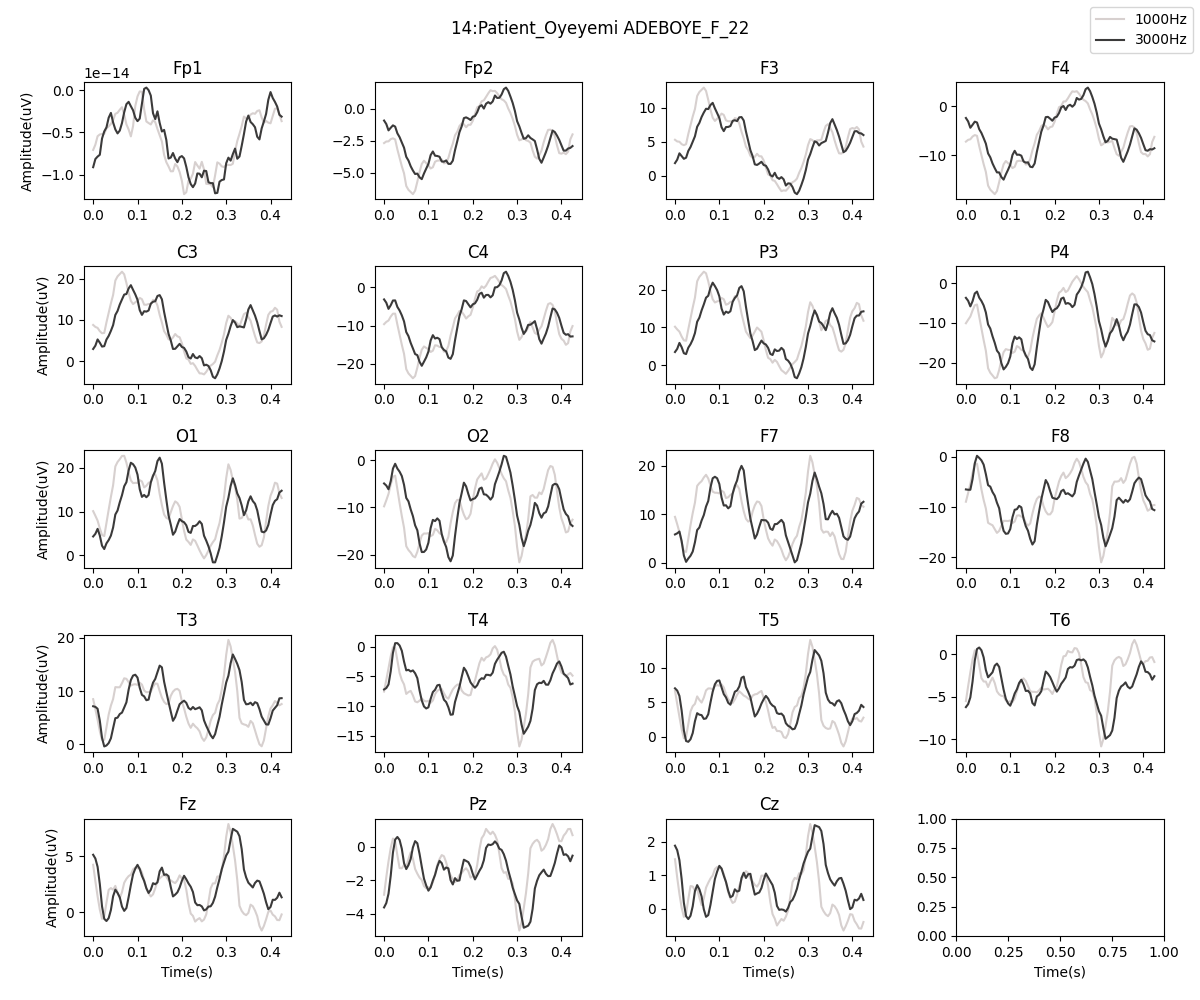
\includegraphics[width=16cm]{../../../data_analysis_results/MMN/time_series/Patient/14.png}
  \caption{A SZ subject MMN plots}
\end{figure}
\begin{figure}[H]
  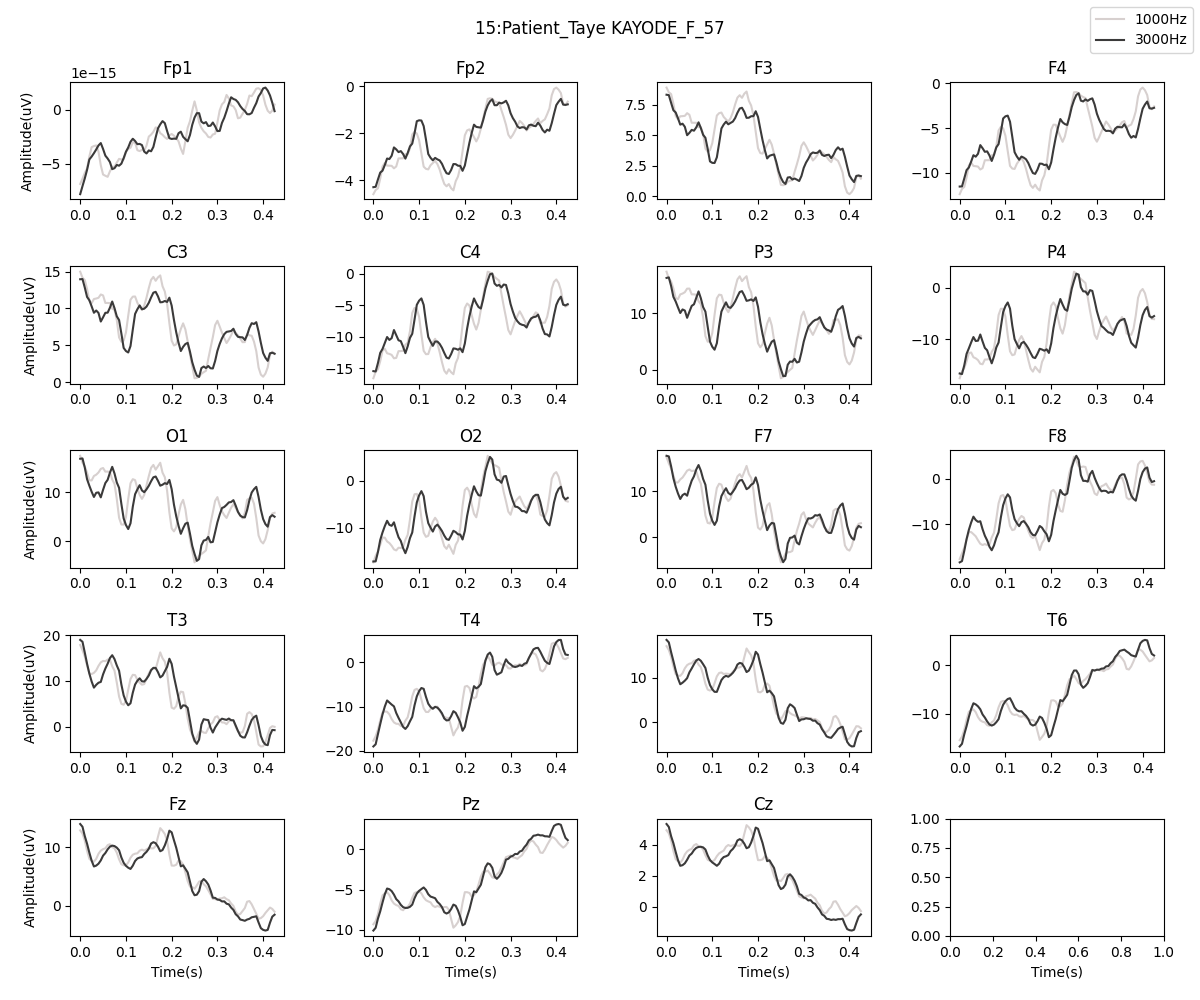
\includegraphics[width=16cm]{../../../data_analysis_results/MMN/time_series/Patient/15.png}
  \caption{A SZ subject MMN plots}
\end{figure}
\begin{figure}[H]
  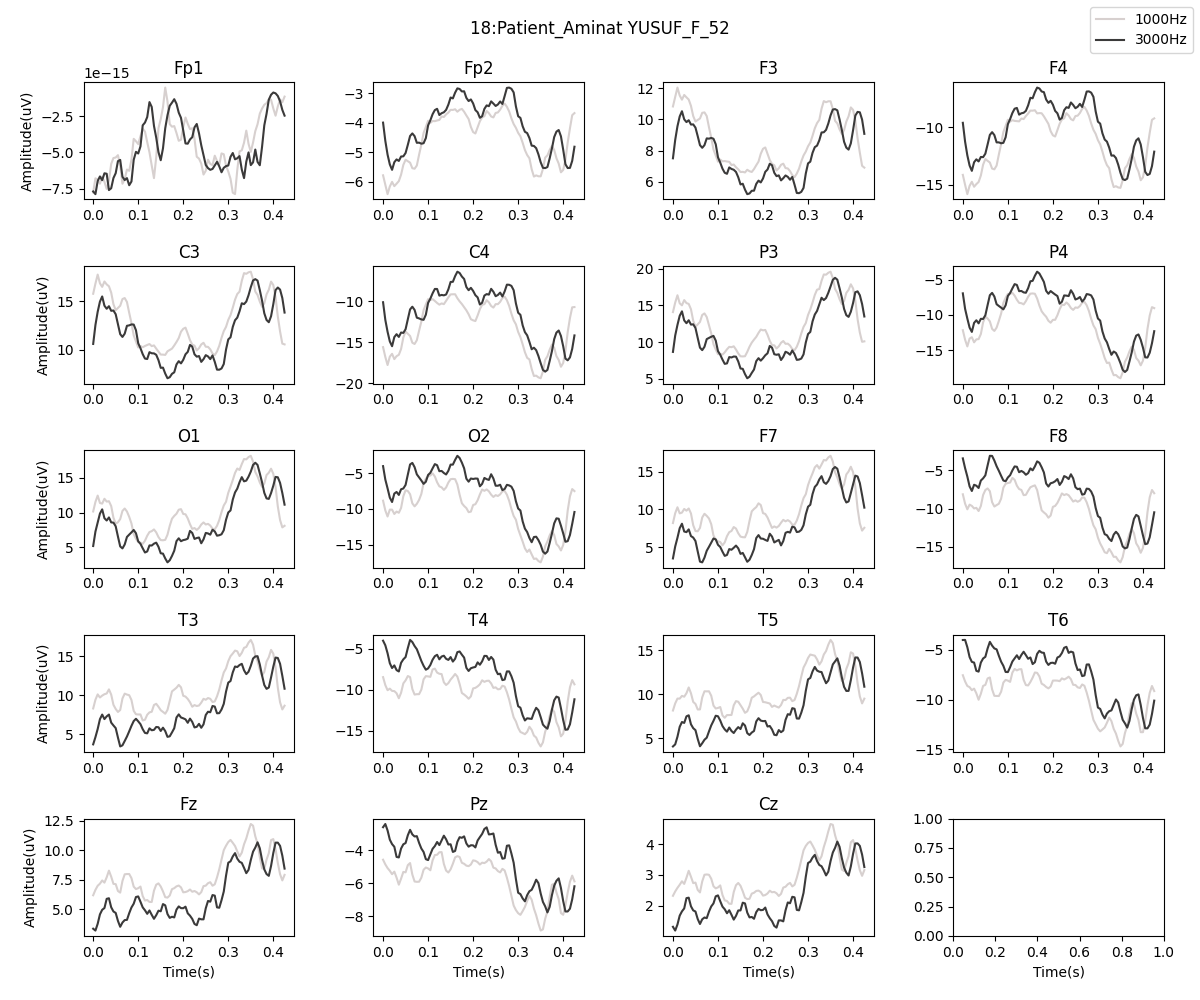
\includegraphics[width=16cm]{../../../data_analysis_results/MMN/time_series/Patient/18.png}
  \caption{A SZ subject MMN plots}
\end{figure}
\begin{figure}[H]
  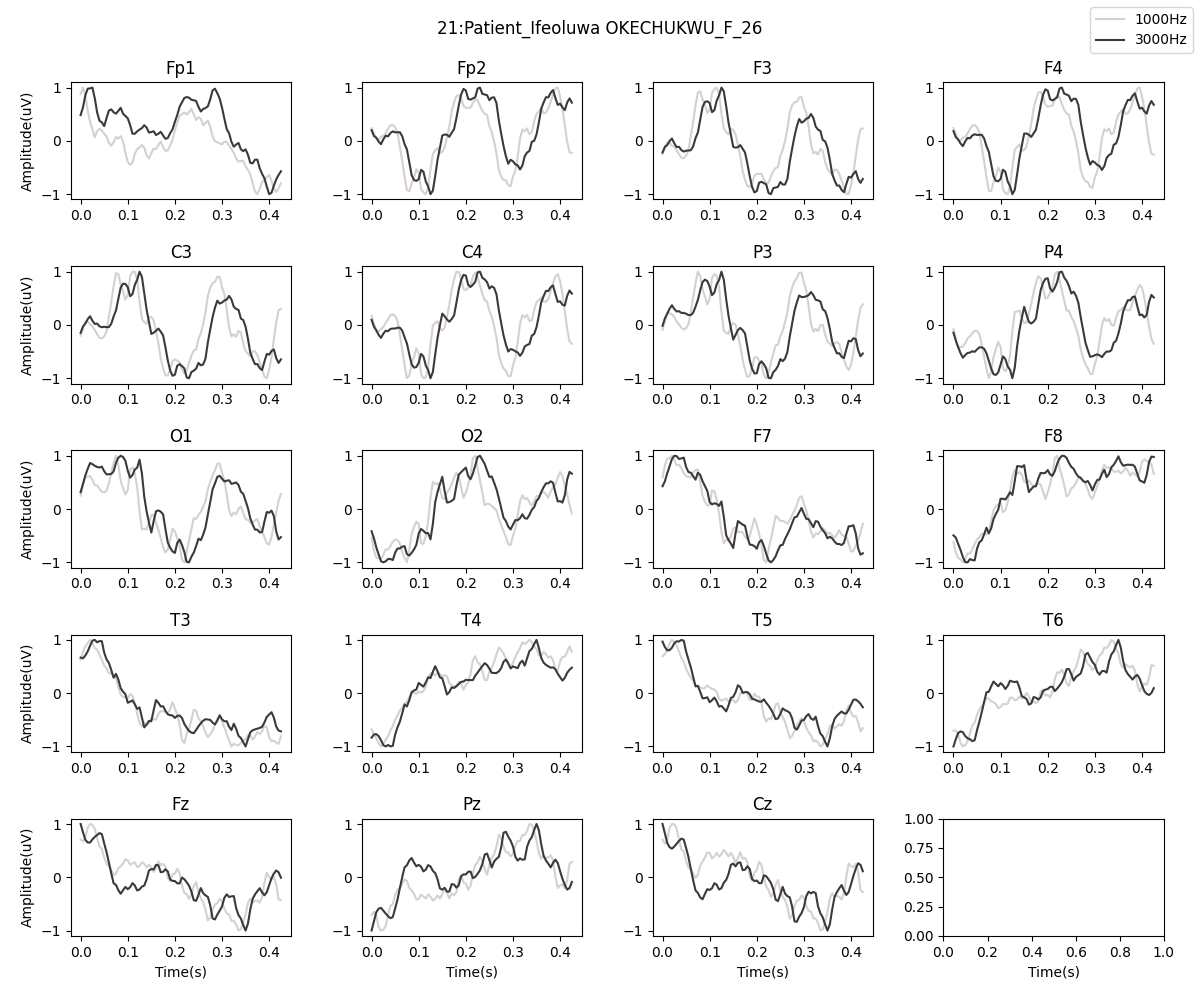
\includegraphics[width=16cm]{../../../data_analysis_results/MMN/time_series/Patient/21.png}
  \caption{A SZ subject MMN plots}
\end{figure}
\begin{figure}[H]
  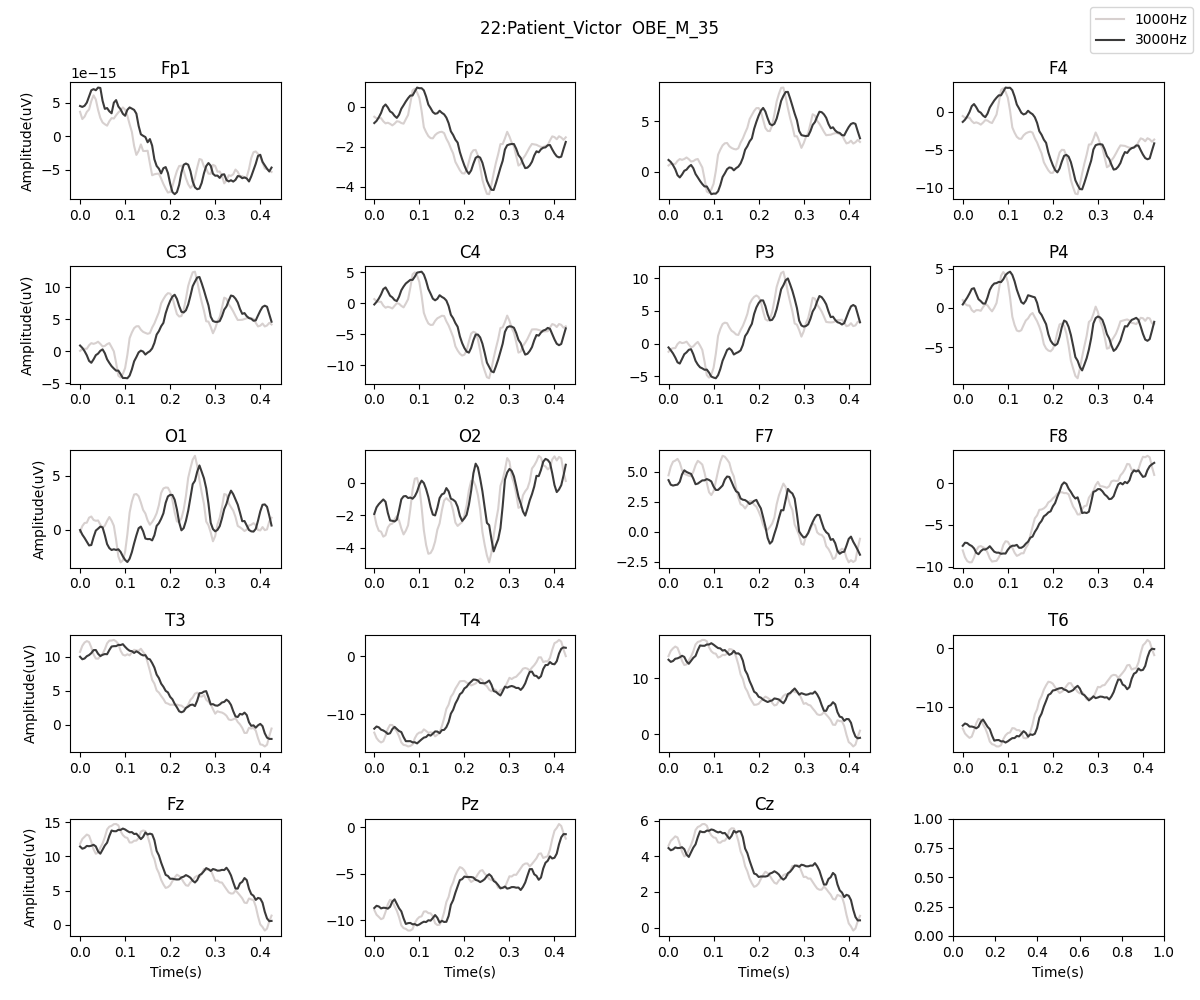
\includegraphics[width=16cm]{../../../data_analysis_results/MMN/time_series/Patient/22.png}
  \caption{A SZ subject MMN plots}
\end{figure}
\begin{figure}[H]
  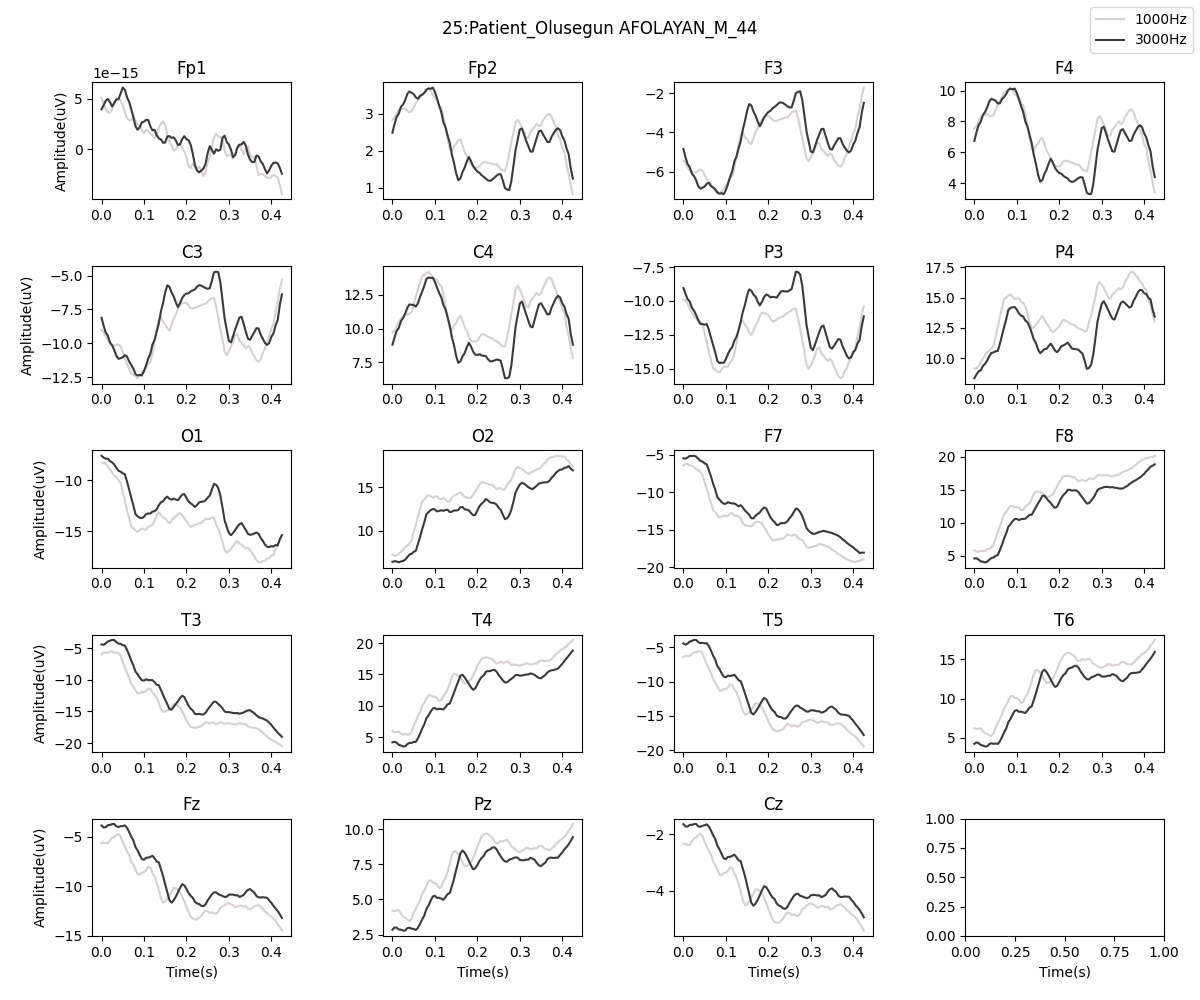
\includegraphics[width=16cm]{../../../data_analysis_results/MMN/time_series/Patient/25.png}
  \caption{A SZ subject MMN plots}
\end{figure}

\clearpage
\section{Appendix}\label{sec:appendix}
\subsection{Fuzzy Entropy Code}
\begin{lstlisting}
import numpy as np
from scipy.spatial.distance import cdist
import time

def sigmoid(x,r):
    assert isinstance(r,tuple), 'When Fx = "Sigmoid", r must be a two-element tuple.'
    y = 1/(1 + np.exp((x-r[1])/r[0]))
    return y  
def default(x,r):   
    assert isinstance(r,tuple), 'When Fx = "Default", r must be a two-element tuple.'
    y = np.exp(-(x**r[1])/r[0])
    return y     
def modsampen(x,r):
    assert isinstance(r,tuple), 'When Fx = "Modsampen", r must be a two-element tuple.'
    y = 1/(1 + np.exp((x-r[1])/r[0]))
    return y    
def gudermannian(x,r):
    if r <= 0:
        raise Exception('When Fx = "Gudermannian", r must be a scalar > 0.')
    y = np.arctan(np.tanh(r/x))    
    y = y/np.max(y)    
    return y    
def linear(x,r):    
    if r == 0 and x.shape[0]>1:    
        y = np.exp(-(x - np.min(x))/np.ptp(x))
    elif r == 1:
        y = np.exp(-(x - np.min(x)))
    elif r == 0 and x.shape[0]==1:   
        y = 0
    else:
        print(r)
        raise Exception('When Fx = "Linear", r must be 0 or 1')
    return y

class fuzzEntropy:
    def __init__(self,window_size,dissimilarity_index,membership_function='linear'):
        self.m = self.window_size = window_size
        self.r = self.dissimilarity_index = dissimilarity_index
        self.mu = self.membership_function = globals()[membership_function.lower()]
    
    def __computeFuzzyMatrix(self,x,m):
        if x.ndim == 1:
            N = x.shape[0]
            Xm = np.array([x[i:i+m-1].tolist() for i in range(0,N-m)])
            dm = cdist(Xm,Xm,'euclidean')
            dm = self.mu(dm,self.r)
            phim = np.sum(dm,axis=1)/(N-m+1)
        return phim
    
    def _fuzzyEntropyCompute(self,x):
        N = x.shape[0]
        phim = self.__computeFuzzyMatrix(x,self.m)
        phim1 = self.__computeFuzzyMatrix(x,self.m+1)

        psim = (1/(N-self.m+1)) * np.sum(phim,axis=0)
        psim1 = (1/(N-self.m+2)) * np.sum(phim1,axis=0)

        with np.errstate(divide='ignore', invalid='ignore'):
            fuzz = np.log(psim)-np.log(psim1)
        return fuzz
    
def fuzzEntropy2D(x,window_size,dissimilarity_index,membership_function=gaussianMembershipfunction):
        fuzzyent = fuzzEntropy(window_size,dissimilarity_index,membership_function)

        res = np.empty(x.shape[0])
        for i in range(x.shape[0]):
            res[i] = fuzzyent._fuzzyEntropyCompute(x[i,:])
        return res.mean()
\end{lstlisting}


\end{document}